\documentclass[12pt]{article}

\usepackage[english]{babel}
\usepackage[utf8x]{inputenc}
\usepackage[T1]{fontenc}
\usepackage{parskip}
\usepackage{lipsum}
\usepackage[a4paper, total={6in, 8in}]{geometry}
\usepackage{setspace}
\usepackage[superscript]{cite}
\usepackage{xcolor}
\usepackage{hyperref}
\usepackage{enumitem}
\usepackage{listings}
\usepackage{amsmath}
\usepackage{amssymb}
\usepackage{ifsym}
\usepackage{tikz}


\begin{document}
	
	
	\begin{flushright}
		\today
	\end{flushright}
	{\Large \textbf{Assignment 10}}
	
	{\large Query Optimization}
	
	\textsc{Ilaria Battiston - 03723403} \\
	\textsc{Mareva Zenelaj - 03736071}
	
	\rule{\linewidth}{0.5pt}
	
	\section{First exercise}
	The initial permutation is $\{R_1, R_2, R_3, R_4, R_5, R_6, R_7, R_8\}$. The first \texttt{for} loop of the algorithm assigns the following numbers to the array $\phi$: $[0, 1, 2, 3, 4, 5, 6, 7]$ with 0 corresponding to $R_1$, 1 to $R_2$ and so on.
	
	Then the algorithm enters the second for loop, changes at each iteration are displayed below:
	\begin{enumerate}
		\item Iteration  1
\\
		Swapping elements 7 and 0
\\
		The new rank is 8
		\item Iteration  2
\\
		Swapping elements 6 and 1
\\
		The new rank is 1
		\item Iteration  3
\\
		Swapping elements 5 and 6
\\
		The new rank is 0
		\item Iteration  4
\\
		Swapping elements 4 and 7
\\
		The new rank is 0
		\item Iteration  5
\\
		Swapping elements 3 and 4
\\
		The new rank is 0
		\item Iteration  6
\\
		Swapping elements 2 and 3
\\
		The new rank is 0
		\item Iteration  7
\\
		Swapping elements 5 and 2
\\
		The new rank is 0
		\item Iteration  8
\\
		Swapping elements 5 and 5
\\
		The new rank is 0
	\end{enumerate}
	The obtained permutation after exiting the loop is $[5, 2, 3, 4, 7, 6, 1, 0]$, corresponding to $\{R_6, R_3, R_4, R_5, R_8, R_7, R_2, R_1\}$.
	
	\section{Second exercise}
	The path on the grid is highlighted in red, using the same number of combinations as the example in Session 10:
	
	\medskip
	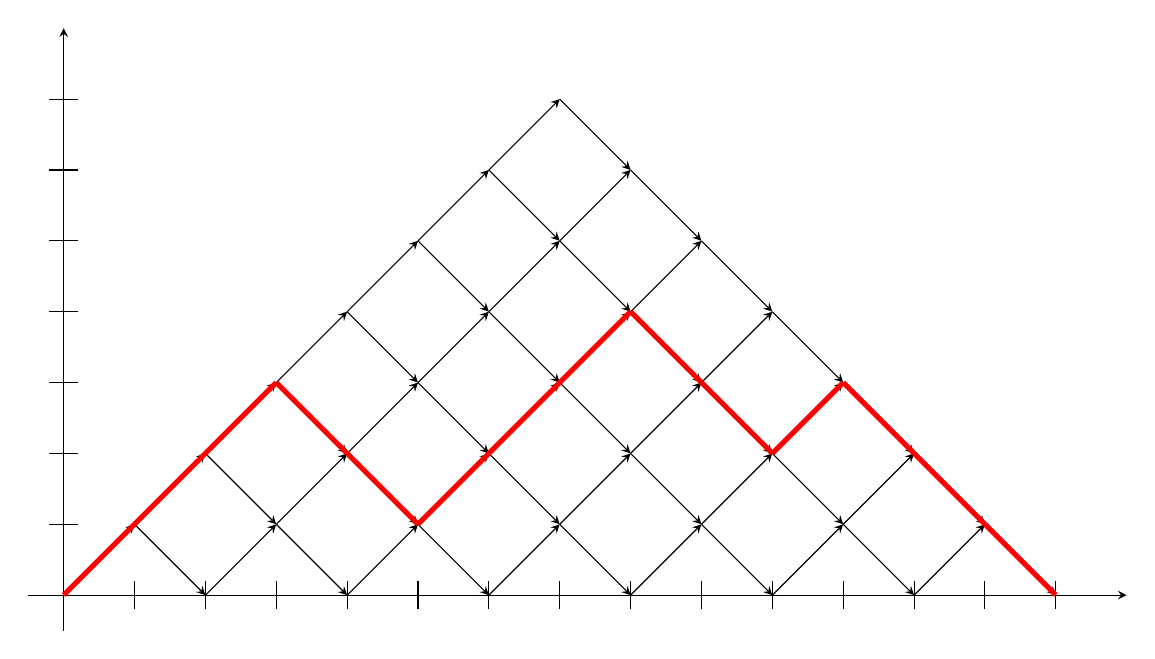
\begin{tikzpicture}[x=9mm,y=9mm]
		\draw[thin,-stealth] (-.5,0) -- (15,0);
		\foreach \xpos in {1,2,...,14}
		\draw[thin] (\xpos,-.2) -- +(0,.4);
		\draw[thin,-stealth] (0,-.5) -- (0,8);
		\foreach \ypos in {1,2,...,7}
		\draw[thin] (-.2,\ypos) -- +(.4,0);
		
		\foreach \x/\y in {
			0/0,2/0,4/0,6/0,8/0,10/0,12/0,
			1/1,3/1,5/1,7/1,9/1,11/1,
			2/2,4/2,6/2,8/2,10/2,
			3/3,5/3,7/3,9/3,
			4/4,6/4,8/4,
			5/5,7/5,
			6/6}{
			\draw[-stealth] (\x,\y) -- +(1,1);
			\draw[-stealth] (\x+1,\y+1) -- +(1,-1);
		}
		\draw[line width=0.65mm, red] (0, 0) -- (1, 1);
		\draw[line width=0.65mm, red] (1, 1) -- (2, 2);
		\draw[line width=0.65mm, red] (2, 2) -- (3, 3);
		\draw[line width=0.65mm, red] (3, 3) -- (4, 2);
		\draw[line width=0.65mm, red] (4, 2) -- (5, 1);
		\draw[line width=0.65mm, red] (5, 1) -- (6, 2);
		\draw[line width=0.65mm, red] (6, 2) -- (7, 3);
		\draw[line width=0.65mm, red] (7, 3) -- (8, 4);
		\draw[line width=0.65mm, red] (8, 4) -- (9, 3);
		\draw[line width=0.65mm, red] (9, 3) -- (10, 2);
		\draw[line width=0.65mm, red] (10, 2) -- (11, 3);
		\draw[line width=0.65mm, red] (11, 3) -- (12, 2);
		\draw[line width=0.65mm, red] (12, 2) -- (13, 1);
		\draw[line width=0.65mm, red] (13, 1) -- (14, 0);
	\end{tikzpicture}

	The order of parentheses is therefore, adding the last right bracket for completeness:
	\texttt{((())((())()))}
	
	From this order we obtain the join tree, with relations from previous permutation added in pre-order:
	
	\begin{tikzpicture}[sibling distance=5cm]
		\node (j1) {$\bowtie$} {
			child {
				node (j2) {$\bowtie$}[sibling distance=6cm]
				child {
					node (j3) {$\bowtie$}[sibling distance=4cm]
					child {
						node (j4) {$R_6$}
					}
					child {
						node (j4) {$R_3$}
					}
				}
				child {
					node (j3) {$\bowtie$}[sibling distance=4cm]
					child {
						node (j4) {$\bowtie$}[sibling distance=5cm]
						child {
							node (j8) {$\bowtie$}[sibling distance=3cm]
							child {
								node (j10) {$R_4$}
							}
							child {
								node (j11) {$R_5$}
							}
						}
						child {
							node (j6) {$\bowtie$}[sibling distance=3cm]
							child {
								node (j00) {$R_8$}
							}
							child {
								node (j11) {$R_7$}
							}
						}
					}
					child {
						node (j4) {$R_2$}
					}
				}
			}
			child {
				node (j7) {$R_1$}
			}
		};
	\end{tikzpicture}
	
\end{document}